 \chapter{Método espectral e Método dos elementos finitos}
\label{cap:I}
\section{Método espectral} 

 Método espectral é um método poderoso usado para solução de equações diferenciais parciais. Diferentemente do método das diferenças finitas, que considera apenas os pontos próximos do ponto que queremos computar chamada de método \emph{local}, o método espectral considera todo o domínio, sendo assim um método \emph{global}. Essa técnica tem mais precisão pois converge exponencialmente diferente do método local. É preferível a utilização desse método quando a solução varia em função do \textit{tempo} e \textit{espaço}. 

\section{Interpolação}
 Para fazer a interpolação da função $f(x)$ por um polinômio trigonométrico ou não, de grau $n$, define-se $P_{n}(x)$ satisfazendo:

\begin{equation}
	P_n (x_i) = f(x_i) \ i = 1,2,...,\emph{n+1}
\end{equation}

 Onde $f(x_i)$ é a função $f$ pré-calculada nos pontos $x_i$. A escolha desses pontos $x_i$ ainda será explicada.

\subsection{Interpolação polinomial}
 \begin{figure}[!ht]
  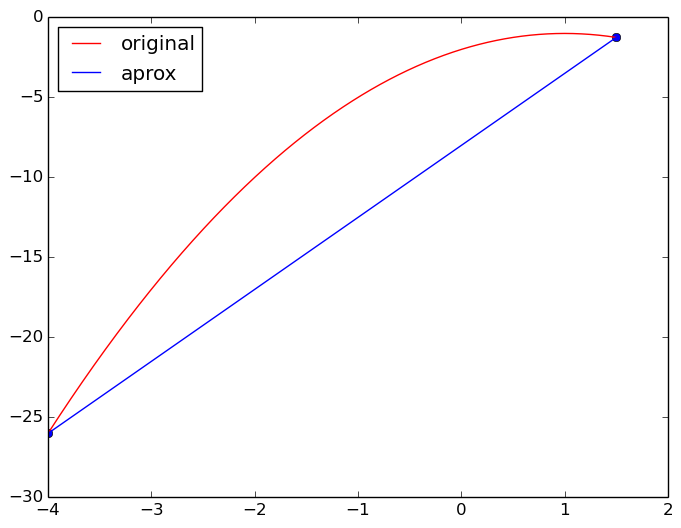
\includegraphics[width=0.7\textwidth,center]{figuras/interpolacao_linear.png}
  \caption{interpolação simples}
\end{figure}

 Antes do uso de calculadoras e computadores, um método de estimar o valor de uma $f$ num ponto,a   maneira mais simples de entender, é a estimação do valor da função em um ponto intermediário entre dois pontos conhecidos é o uso da interpolação \emph{Linear}.

\begin{equation}
	f(x) \approx \frac{x - x_1}{x_0 - x_1}f(x_0)  + \frac{x - x_0}{x_1 - x_0}f(x_1)
\end{equation} 
 
 Para fazermos essa interpolação para $n$ pontos conhecidos aproximamos uma função usando o polinômio base de \emph{Lagrange}.
\begin{equation}
C_i(x) = \prod_{j = 0 \\ j \neq i}^{N} \frac{x - x_j}{x_i - x_j} 
\end{equation} 

\begin{figure}[!h]
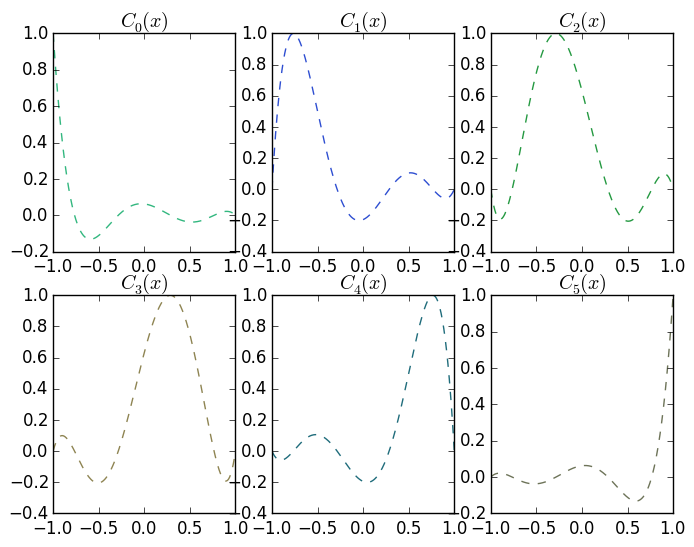
\includegraphics[width=0.7\textwidth, center ]{figuras/exemplo_polinomio_lagrange.png}
\caption{polinômio base de Lagrange para 6 pontos}
\end{figure}

 A interpolação de \emph{Lagrange} é dada por :
\begin{equation}
 P_n(x) \equiv \sum_{i = 0}^{N} f(x_i)C_i(x) 
\end{equation}    
 Com isso,  a interpolação é tal que $P_n(x_i) = f(x_i)$. Apesar dos pontos interpoladores equidistantes serem comumente utilizados, não há restrições, podendo até mesmo estar fora de ordem.
\begin{figure}[h]
  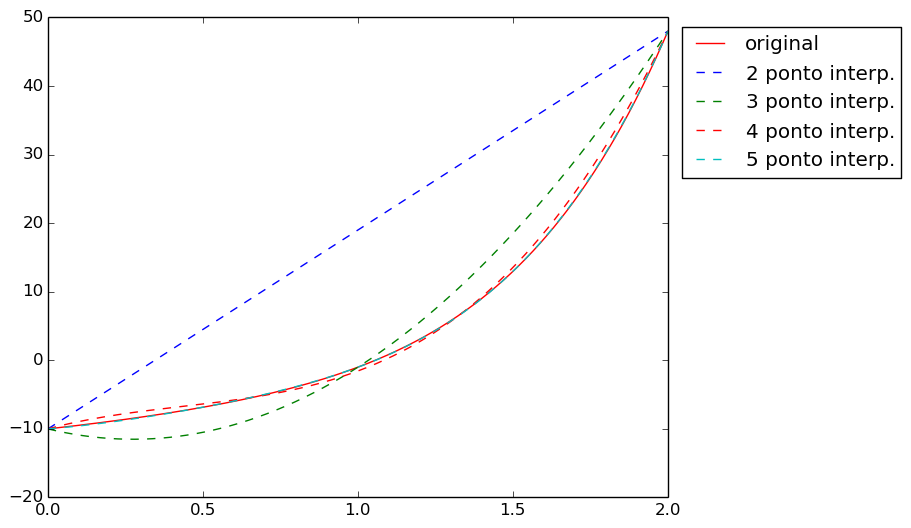
\includegraphics[width=0.5\textwidth, center]{figuras/interpolacao_linear5.png}
  \caption{interpolação com n pontos equidistantes}
\end{figure}

\pagebreak
\newpage

\subsection{Fenômeno de Runge}
 Apesar de parecer que uma boa interpolação tenha uma boa aproximação usando pontos igualmente espaçados sobre um interval $[a,b]$, $\lim_{n \to \infty} |f(x) - P_n(x)| = 0$ para qualquer $f(x)$ diferenciável., isto nem sempre é verdade. No início do século XX, \emph{Carl David Tolmé Runge}, provou para a função $f(x)$:
 \begin{equation}
 f(x) = \frac{1}{1 + x^2} , x \in [-5,5]
 \end{equation}
 que para pontos equidistantes, a interpolação converge apenas no intervalo $[-3.63,3.63]$, e diverge fora do mesmo. Para polinômios de maior grau, esse intervalo de convergência tende a diminuir e perto dos pontos de fronteira diverge bastante (figura abaixo).

\begin{figure}[htp]
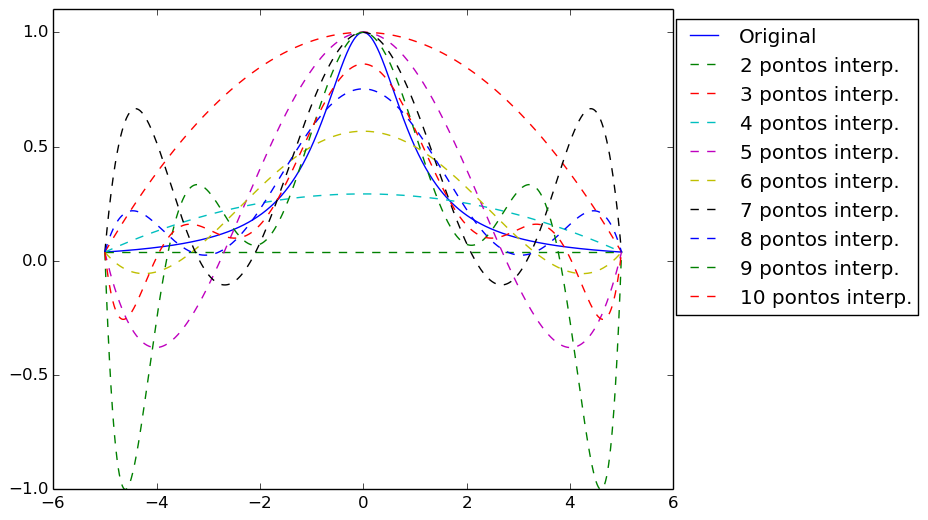
\includegraphics[width=0.7\textwidth, center]{figuras/fenomeno_runge.png}
\caption{fenômeno Runge}
\end{figure}

 Assim, Runge prova que no meio do intervalo temos boas aproximações mas infelizmente perto dos extremos, os valores interpolados oscilam muito, para um polinômio de grau n com pontos equidistante. Esse fenômeno sugere que escolhamos pontos diversos que tenham menor concentração no meio do intervalo, onde temos uma maior precisão, e aumentar a densidade de pontos próximos dos extremos.
 Agora como encontrar uma distribuição de pontos de forma que melhore a interpolação? A resposta pode ser explicado pelos teoremas a seguir.
\pagebreak
\subsection{ Teorema I: Erro de interpolação de Cauchy}

 Dado $f(x)$  com pelo menos $N+1$ derivadas no intervalo de interesse e seja $P_N(x)$ seja o interpolador Lagrangiano de grau $N$. Então o erro é dado por:
 
 \begin{equation}
 f(x) - P_{N+1}(x) = \frac{1}{[N+1]!}f^{(N+1)}(\epsilon)\prod^{N}_{i = 0} (x - x_i)
 \end{equation}
 Para um $\epsilon(x) \in [-1,1]$.
 
 Logo, para minimizar o erro, não podemos fazer nada quanto ao termo $f^{(N+1)}(\epsilon)$, pois para isso  necessitamos conhecer a função interpolada. Quanto ao polinômio $\prod^{N}_{i = 0} (x - x_i)$, sabemos que expandindo o produtório, o coeficiente do termo $x^N$ é $1$, independente da escolha de pontos. Então a pergunta que fica é, qual escolha de pontos que nos dá um \emph{polinômio} com coeficiente líder igual a $1$ minimiza essa função ? Felizmente e coincidentemente, essa resposta foi respondida quase meio século antes do próprio fenômeno de Runge ser descoberto. Veremos no próximo teorema.

 
\subsection{Teorema II: Amplitude minima} \label{subsec:TeoremaII}
 De todos os polinômios de grau $N$ com coeficiente de $x^N$ igual a 1, o único polinômio que tem o menor máximo no intervalo $[-1,1]$ é $\frac{T_N(x)}{2^{N-1}}$, o polinômio de \emph{Chebyshev}  dividido por $2^{N-1}$. Em outras palavras, todos os polinômios de mesmo grau e coeficiente líder unitário,chamados de polinômios mônicos, satisfazem a desigualdade:

\begin{equation}
	max_{x \in [-1,1]}|P_N(x)| \geq  max_{x \in [-1,1]} \left |\frac{T_N(x)}{2^{N-1}}  \right |  = \frac{1}{2^{N-1}}\\
\end{equation}

\begin{align}
    &T_0(x) = 1\\
    &T_1(x) = x\\
    &T_{N+1}(x) = 2xT_N(x) - T_{N-1}(x)\\
    &T_{N}(x) =\cos(n \arccos x)=\cosh(n\,\operatorname{arcosh}\,x)
\end{align}

 Agora, qualquer polinômio de grau $N$, com coeficiente líder unitário, pode ser fatorado na forma de um produtório  $(x - x_i)$, onde $x_i$ é uma das raízes do polinômio, em particular: 
 \begin{equation}
 \frac{1}{2^N}T_{N+1}(x) \equiv \prod_{i = 1}^{N+1} (x-x_i)
 \end{equation}
 Temos então que, para minimizar o erro no \emph{Teorema I}, o polinômio deve ser proporcional a $T_{N+1}(x)$. Isso implica que  os pontos interpoladores que minimizam o erro, são as raízes do próprio polinômio de \emph{Chebyshev} de grau $N+1$.
 
 Usando o fato que esse polinômio pode ser reescrito como uma função trigonométrica, temos que as raízes são:
 \begin{equation}
  x_i  \equiv \cos \left [ \frac{(2i - 1)\pi}{2(N+1)}  \right ] , i = 1,2,..., N+1
 \end{equation}
 
 Pela expansão de \emph{Taylor} da função coseno, verificamos que segundo   a definição de $x_i$ acima, o espaçamento da malha é $O(N^2)$ perto das fronteiras:
 
 \begin{equation}
  x_1 \approx -1 + \frac{\pi^2}{8N^2}\ ;\ x_2 \approx -1 + \frac{9\pi}{8N^2}\ \ [N\gg 1]
 \end{equation}
 
 Agora temos como conseguir o polinômio de \emph{Chebyshev} que minimiza o erro. Porém essa escolha de polinômio varia para diferentes geometrias no $\mathbb{R}^2$ ou funções harmônicas ou hermitianas.
 \begin{figure}[t]
 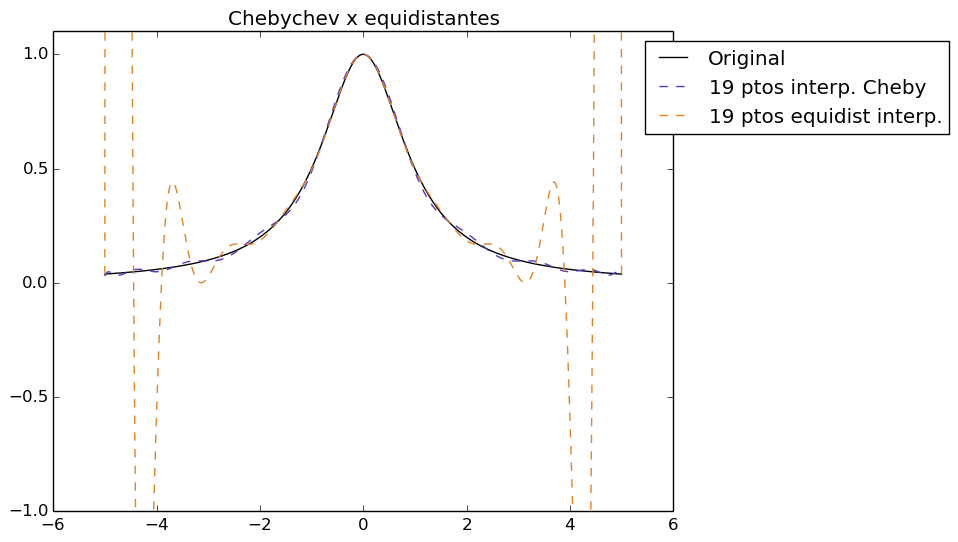
\includegraphics[width=0.7\textwidth, center]{figuras/chebychev_equidist.png}
 \caption{método de raízes de Chebychev contra raízes de pontos equidistante}
 \end{figure}
\pagebreak
\section{Integração numérica pelo método de colocação }
 Usando os polinômios interpoladores $P_i$ de uma mesma família qualquer,  de grau menor ou igual a $n$, podemos escrever a integral de $f$ no intervalo $[a,b]$:
 
\begin{equation}
\int^{a}_b f(x) \partial x\ = \int^{a}_b[\sum_{i\ =\ 0}^N P_i(x) f(x_i)]\ \partial x +  \int^{a}_b \prod_{i\ =\ 0} (x - x_i)\frac{f^{(n+1)}(\varepsilon)}{(n+1)!}\ \partial x\\
\end{equation}

podemos aproximar a integral por:
\begin{equation}\label{eq:integra}
   \int^{a}_b f(x) \partial x\ \approx \sum_{i\ =\ 0}^N f(x_i) \int^{a}_b P_i(x) \partial x\ =\ \sum_{i\ =\ 0}^N f(x_i) w_i \\
\end{equation}

onde o coeficiente é:
\begin{equation}
 w_i =  \int^{a}_b  P_i(x) \partial x
\end{equation}
 para demonstrarmos que o termo de \emph{erro} na equação \eqref{eq:integra}, é zerada, fazemos a seguinte prova:\\
 Tomando $f$ como sendo um polinômio de grau $(2n+1)$, temos que $f^{(n+1)}$ será um polinômio de grau $n$. Logo, reescrevendo $f^{(n+1)}$, temos:
 \begin{equation}
 f^{(n+1)}(x) = \sum^{n-1}_{j = 0} b_j P_j(x)
 \end{equation}
 E também para interpolar o termo $\prod^{n}_{i = 0} (x - x_j)$:
\begin{equation}
 \prod^{n}_{i = 0} (x - x_j) =  P_{n+1}(x)
\end{equation}  
Assim, fazemos:
\begin{equation}
\int^{a}_b \prod_{i\ =\ 0} (x - x_i)\frac{f^{(n+1)}(\varepsilon)}{(n+1)!}\ \partial x = \sum^{n-1}_{j = 0} b_j \int^{a}_b   P_{n+1}(x) P_j(x) \partial x
\end{equation}
 Agora, sejam os polinômios $P_i$'s ortogonais em relação ao produto escalar:
\begin{equation}
 (f,g) = \int^b_a f(x)g(x) \partial x
\end{equation}
 Assim anulamos o erro:
\begin{align}
&(P_i,P_j) = \int^b_a P_i(x) P_j(x) \partial x = 0\ ,\ i \neq j\\
&\int^{a}_b \prod_{i\ =\ 0} (x - x_i)\frac{f^{(n+1)}(\varepsilon)}{(n+1)!}\ \partial x = \sum^{n-1}_{j = 0} b_j \int^{a}_b   P_{n+1}(x) P_j(x) \partial x = 0
\end{align}
 No caso acima foi utilizado para a integração um polinômio qualquer ortogonal, porém podemos utilizar qualquer classe de polinômios \emph{ortogonais} para estimarmos a integral da função, tomando os zeros dos polinômios a nossa escolha.[\emph{Gauss-Chebychev}, \emph{Gauss-Jacobi}, \emph{Gauss-Radau}, \emph{Gauss-Lobatto}]
 
\section{Derivação pelo método da colocação }
 Com a interpolação de $f(x) \in P_p$, onde $P_p$ é o espaço de polinômios de grau $\leq p$,  ela pode ser reescrita em termos de polinômios de Lagrange $C_i$, por $N + 1$ e $x \in -1 \leq x \leq 1$ pontos como:
 \begin{equation}
 f(x)  = \sum^{N}_{0} f(x_i) C_i(x)
 \end{equation}
 A derivada da $f(x)$ é dada por:
 \begin{equation}
 \frac{\partial f(x)}{\partial x} = \sum^{N}_{i = 0} f(x_i) \frac{\partial C_i(x)}{\partial x}
 \end{equation}
 Calculando $\frac{\partial f(x)}{\partial x}$ nos pontos nodais $x_i$, temos:
\begin{equation}
   \frac{\partial f(x)}{\partial x}  \Biggm\lvert_{x=x_i} = \sum^{N}_{j\ = 0} f(x_j) C_{ij}
\end{equation}
 Onde:
 \begin{equation}
  C_{ij} = \frac{\partial C_i(x)}{\partial x} \Biggm\lvert_{x=x_i}
 \end{equation}
 a derivada de $C_i(x)$ é:
 \begin{align}
 &C_i(x) = \frac{P_{n+1}(x)}{P'_{n+1}(x)(x -\ x_i)}\ ,\ P_{n+1}(x) = \prod^{N}_{0} (x - x_j)\\
 &\frac{\partial C_i(x)}{\partial x} =  \frac{P'_{n+1}(x)(x\ -\ x_i) - P_{n+1}(x)}{P'_{n+1}(x)(x - x_i)^2}\ 
 \end{align}
 temos que para x tendendo para $x_i$:
 \begin{equation}
 \lim_{x \rightarrow x_i}  \frac{\partial C_i(x)}{\partial x} =  \lim_{x \rightarrow x_i} \frac{P''_{n+1}(x)}{2P'_{n+1}(x)} = \frac{P''_{n+1}(x_i)}{2P'_{n+1}(x_i)}
 \end{equation}
 assim, ficamos com:
 \begin{equation}\label{eq:test}
 C_{ij}= 
\begin{cases}
    \frac{P'_{n+1}(x_i)}{P'_{n+1}(x_j)} \frac{1}{(x_i - x_j)},& \text{se}\ i\ \neq  j\\\\
    \frac{P''_{n+1}(x_i)}{2P''_{n+1}(x_j)},              & \text{caso contrário}
\end{cases}
 \end{equation}
 Matricialmente podemos fazer:
\begin{equation}
 U'= \begin{bmatrix} 
u'(x_0)\\ 
u'(x_1)\\
...\\
u'(x_N)\\ 
\end{bmatrix} =
\begin{bmatrix}
C_{00} &   C_{01} & \ldots & C_{0N}\\
C_{10}  &  C_{11} & \ldots & C_{1N}\\
\vdots & \vdots & \ddots & \vdots\\
C_{N0}  &   C_{N1}       &\ldots & C_{NN}
\end{bmatrix}. \begin{bmatrix} 
u_{0}\\ 
u_{1}\\
\vdots\\
u_{N}\\ 
\end{bmatrix} 
\end{equation}  
  Para a mudança de intervalo $ x \in [-1,1]$ para $y \in [a,b]$ podemos fazer:
\begin{align}
&y = \frac{(1-x)}{2}a + \frac{(1+x)}{2}b \\
&\frac{\partial y}{\partial x} = \frac{(b -a)}{2}\\
&\frac{\partial f}{\partial x} = \frac{\partial f}{\partial y}. \frac{\partial y}{\partial x} \\
&\frac{\partial f}{\partial y} =  (\frac{\partial y}{\partial x})^{-1}.\frac{\partial f}{\partial x} \\
&\frac{\partial f}{\partial y} = \frac{2}{(b -a)}.\frac{\partial f}{\partial x}
\end{align}
  
\subsection{Polinômios de Jacobi}
 Polinômios de Jacobi $P^{\alpha,\beta}_n(x)$ são famílias de polinômios de soluções para problemas de \emph{Sturm-Liouville}. Tais polinômios são \emph{ortogonais} no intervalo $[-1,1]$  com respeito funções peso do tipo $(1-x)^\alpha (1+x)^\beta$ para $\alpha,\beta > -1$.
Pela fórmula de Rodrigues, essa família é dada por:
\begin{equation}
P_n^{(\alpha,\beta)}(x) = \frac{(-1)^n}{2^n n!} (1-x)^{-\alpha} (1+x)^{-\beta} \frac{d^n}{dx^n} \left\{ (1-x)^\alpha (1+x)^\beta \left (1 - x^2 \right )^n \right\},\ (\alpha, \beta >-1)
\end{equation}
 sua derivada é dada por:
\begin{equation}
\frac{\partial P^{\alpha,\beta}_n (x)}{\partial x} = \frac{1}{2}(n+\alpha+\beta) P^{\alpha + 1,\beta +1}_{n-1} (x)
\end{equation}
 onde podemos encontrar $P^{\alpha + 1,\beta +1}_{n-1}$ pela relação recursiva:
\begin{align}
& P^{\alpha,\beta}_{0} (x) = 1\\
& P^{\alpha,\beta}_{1} (x) = \frac{1}{2}[\alpha - \beta + (\alpha + \beta + 2 )x]\\
& P^{\alpha,\beta}_{n+1} (x)=(a^2_n + a ^3_n x)P^{\alpha,\beta}_{n}(x) - a_n^4P^{\alpha,\beta}_{n-1}(x)  \\
& a^1_n = 2(n+1)(n+ \alpha + \beta + 1)(2n + \alpha +\beta)\\
& a^2_n = (2n + \alpha +\beta + 1)(\alpha^2 - \beta^2)\\
& a^3_n = (2n + \alpha +\beta)(2n + \alpha +\beta + 1)(2n + \alpha + \beta + 2)\\ 
\end{align}
 Anteriormente utilizado nos exemplos, o polinômio de \emph{Chebyshev} e o conhecido polinômio de \emph{Legendre} são na verdade um caso especial do polinômio de \emph{Jacobi}:
\begin{align}
& \text{Polinômio de Chebychev} (\alpha= \beta = -\frac{1}{2})  \rightarrow  T_n(x) =\frac{2^{2n}(n!)^2}{ (2n)!} P^{(-\frac{1}{2},-\frac{1}{2})}_{n}(x) \\
& \text{Polinômio de Legendre} (\alpha= \beta = 0)  \rightarrow L_n(x) =  P^{(0,0)}_{n}(x)
\end{align}
 
 \emph{Interpolador de Gauss-Lobatto}: Nesse caso, os pontos de interpolação são os zeros do polinômio $[P^{\alpha,\beta}_{Q-2}(x)]'$. E a derivada da função é dada por:
\begin{equation}
 C_{ij}= 
\begin{cases}
 \frac{(-1)^{Q - 1}(Q-2)!\Gamma(\beta +2)}{(Q + \alpha + \beta)\Gamma(Q + \beta)}(x-1)[P^{\alpha,\beta}_{Q-1}(x)]'\  \  \ \text{se}\  j = 0 \\\\
 \frac{(x^2 -1)[P^{\alpha,\beta}_{Q-1}(x)]'}{(Q-1)(Q + \alpha + \beta)P^{\alpha,\beta}_{Q-1}(x)(x-x_j)} \text{se}\  1 \leq j \leq Q-2\\\\
 \frac{(x^2 -1)[P^{\alpha,\beta}_{Q-1}(x)]'}{(Q + \alpha + \beta)\Gamma(Q+\alpha)}(x+1)[P^{\alpha,\beta}_{Q-1}(x)]' \ \ \text{se} \ \ j = Q - 1
\end{cases}\\
\end{equation} 
\\
 \emph{Gauss-Radau-Jacobi}: Esse caso, só consideramos o extremo da esquerda [-1] e os pontos internos:
 \begin{equation}
 x_{i}= 
\begin{cases}
 -1 \ i = 0\\
 x^{\alpha,\beta +1}_{i-1,N-1}(x) \ i= 1,...,N-1\\
\end{cases}\\
 \end{equation}
 E é dada por :
 \begin{align}
  & P_{N}(x) = (1+x)P^{\alpha,\beta+1}_{N -1}(x)\\
  & P'_{N}(x) = (1+x)[P^{\alpha,\beta+1}_{N -1}(x)]' + P^{\alpha,\beta+1}_{N -1}(x)\\
  & P''_{N}(x) = (1+x)[P^{\alpha,\beta+1}_{N -1}(x)]'' + 2P^{\alpha,\beta+1}_{N -1}(x)
 \end{align}
 Calculando nos pontos internos:
 \begin{align}
  & P'_{N}(x_i)= 
\begin{cases}
 \frac{-1^{N-1}\Gamma(N+\beta+1)}{\Gamma(N)\Gamma(\beta+2)} \ i =0\\ \\
 (1+x_i)[P^{\alpha,\beta+1}_{N -1}(x)]' \ \ \ i= 1,...,N-1\\ 
\end{cases}\\ \\
  & P''_{N}(x_i)= 
\begin{cases}
 \frac{-1^{N} (N+\alpha+\beta+1)}{\Gamma(N-1)\Gamma(\beta+3)} \ i =0\\  \\
 \frac{(\alpha -\beta +1+(\alpha+\beta+1)x_i)}{(1-x_i)}[P^{\alpha,\beta+1}_{N -1}(x)]' \ \ i= 1,...,N-1\\
\end{cases}\\
 \end{align}\\
\emph{Gauss-Lobatto-Jacobi}: nesse caso, consideramos ambos os extremos (-1 e +1):
\begin{equation}
 x_{i}= 
\begin{cases}
 -1 \ i = 0\\
 x^{\alpha,\beta +1}_{i-1,N-1}(x) \ i= 1,...,N-2\\
  1 \ i = N-1
\end{cases}\\
\end{equation}
 E assim:
 \begin{align}
  & P_{N}(x) =   (1-x)(1+x)P^{\alpha+1,\beta+1}_{N -2}(x)\\
  & P'_{N}(x) =  (1-x)(1+x)[P^{\alpha+1,\beta+1}_{N -2}(x)]' -  2P^{\alpha+1,\beta+1}_{N -2}(x)\\
  & P''_{N}(x) = (1-x)(1+x)[P^{\alpha+1,\beta+1}_{N -2}(x)]'' -4x[P^{\alpha+1,\beta+1}_{N -2}(x)]' - 2P^{\alpha,\beta+1}_{N -1}(x)
 \end{align}
 E calculando as derivadas:
 \begin{align}
  & P'_{N}(x_i)= 
\begin{cases}
 \frac{-1^{N}2\Gamma(N+ \beta)}{\Gamma(N-1)\Gamma(\beta+2)} \ i =0\\ \\
 (1+x_i)(1-x_i)[P^{\alpha+1,\beta+1}_{N-2}(x_i)]' \ \ \ i= 1,...,N-2\\ 
 \frac{-2\Gamma(N+\alpha)}{\Gamma(N-1)\Gamma(\alpha +2)} \ \ i = N-1
\end{cases}\\ \\
  & P''_{N}(x_i)= 
\begin{cases}
 \frac{(-1)^N 2(\alpha -(N-1)(Q+\alpha+\beta)))}{\beta + 2}\frac{\Gamma(N+\beta)}{\Gamma(N-1)\Gamma(\beta + 2)}\ i =0\\  \\
(\alpha -\beta +1+(\alpha+\beta)x_i)[P^{\alpha+1,\beta+1}_{N-2}(x_i)]'\ \ i= 1,...,N-2\\
\frac{2(\beta -(N-1)(N + \alpha + \beta))}{\alpha + 2}\frac{\Gamma(N+\alpha)}{\Gamma(N-1)\Gamma(\alpha+2))} \ \ i = N-1
\end{cases}\\
 \end{align}\\
 onde $\Gamma(x)$ é a função gamma.

\section{Método dos resíduos ponderados}
 A fim de resolvermos a equação diferencial, temos que tornar a solução $u^\delta(x)$ aquela que melhor aproxima a solução exata do problema $u(x)$, para isso devemos então minimizar o resíduo dessa aproximada. Tomando o problema diferencial abaixo, temos o operador diferencial $L(\bullet)$
 \begin{align}
     L(u) &= \frac{\partial^2 u}{\partial x^2} + \lambda u + f = 0 \\
    L(u) &= 0
 \end{align}

 Aproximando $u$ por $u^\delta$ obtemos um erro associado ao operador $L(\bullet)$:
 \begin{equation}
 	u^\delta(x) = u(x_0) + \sum^{N_{dof}}_{i = 1} u(x_i) \Phi(x)\\
    L(u^\delta) = R(u^\delta)
\end{equation}
Nosso problema está na minimização desse erro $R(u^\delta)$. Para isso, escolhemos uma função teste $v_j$ onde $j = 1,2,\dots, N_{dof}$, tal que seu produto interno com o erro seja o menor possível.
\begin{equation}
    <v_j,R(u^\delta)> = \int_{\Omega} v_j(x)\ R(x) \partial x,\ \forall j = 1,2,3,\dots,N_{dof}\\
\end{equation}
Assim, obtemos um sistema linear para cada j no qual escolhido a melhor função teste $v_j$, temos a melhor aproximação $u^\delta$. Ao longo dos anos várias funções foram encontradas para a minimização dos erros. O método mais conhecido é o dos Mínimos Quadrados no qual $v_j\ =\ \frac{\partial R}{\partial \hat{u}_j}$. Alguns outros também existem como o método de \emph{colocação} e método dos \emph{momentos}. Aquele que usarei é o método de \emph{Galerkin}, onde escolhemos $v_j \equiv \phi_j$ e $v_j(\Omega_d) = 0$ onde $\Omega_d$ é a fronteira de \emph{Dirichlet}.

\section{Método de Galerkin}
 O método de \emph{Galerkin}, também conhecido como \emph{Bubnov-Galerkin} devido a Ivan Grigoryevich Bubnov  e Boris Grigoryevich Galerkin  será o mais utilizado daqui pra frente. Para fins de exemplo consideramos a seguinte equação diferencial em uma dimensão:
 \begin{equation}\label{eq:eq_dif}
 L(u) \equiv \frac{\partial^2 u}{\partial x^2} + f = 0
 \end{equation}
 
 Para esse problema ser bem posto e então obter uma solução única, precisamos especificar as condições de fronteira num domínio $\Omega = \{x| -1 < x < 1\}$, assim sendo temos:
 \begin{equation}
 u(-1)=g_D\ ,\ \frac{\partial u(1)}{\partial x} = g_N
 \end{equation}
 Onde $g_D$ e $g_N$, são constantes, e são chamadas de condição de contorno de \emph{D}irichlet e \emph{N}eumman. Essas condições junto da equação \eqref{eq:eq_dif}, chamamos essa combinação como formulação \emph{Forte} do problema.
\subsection{Formulação fraca e a implementação da condição de fronteira de Neumman}
 Multiplicando a equação \eqref{eq:eq_dif}, por uma função $v(x)$, que por definição é 0 na fronteira de \emph{Dirichlet} $\partial \Omega_D$, e integrando sobre o domínio $\Omega$, obtemos o produto interno de $L(u)$ e $v$:
 \begin{equation}\label{eq:eq_fraca}
 (v,L(u))=\int^1_{-1} v\left ( \frac{\partial^2u}{\partial x^2} + f \right )\partial x = 0
 \end{equation}
 Podemos ver que essa equação \eqref{eq:eq_fraca} pode ser reescrita usando integração por partes obtemos:
 \begin{align}
& \int^{1}_{-1} v \frac{\partial^2 u}{\partial x^2} \partial x = \left [ v\frac{\partial u}{\partial x}    \right ]^{1}_{-1} - \int^{1}_{-1} \frac{\partial v}{\partial x}  \frac{\partial u}{\partial x}  \partial x \\
&  \int^{1}_{-1} \frac{\partial v}{\partial x}  \frac{\partial u}{\partial x}  \partial x =  \int^{1}_{-1}  v f\ \partial x  + \left [ v\frac{\partial u}{\partial x}    \right ]^{1}_{-1} 
 \end{align}
 Como a função teste $v$ é zero na fronteira de \emph{Dirichlet}, sabemos que $v(-1) = 0$. Assim, aplicando a condição de fronteira de \emph{Neumman}, $\frac{\partial u(1)}{\partial x} = g_N$, simplificamos a equação, temos:
 \begin{equation}
 \int^{1}_{-1} \frac{\partial v}{\partial x}  \frac{\partial u}{\partial x}  \partial x =  v(1)g_N + \int^{1}_{-1}  v f\ \partial x  
\end{equation}

Vemos que nessa última etapa, a condição de fronteira de \emph{Neumman} é naturalmente inclusa na formulação. A forma integral da equação como vimos nas últimas duas etapas, é dita como a \emph{Formulação Fraca} do problema.

A solução aproximada de Galerkin da equação \eqref{eq:eq_dif}, é a solução para a formulação fraca da equação, quando a solução exata $u(x)$ e a função teste $v(x)$ são aproximadas por expanções \emph{finitas} $u^\delta(x)$ e $v^\delta(x)$, e assim a  equação diferencial se torna:
\begin{equation}\label{eq:eqdif_neumann}
 \int^{1}_{-1} \frac{\partial v^\delta}{\partial x}  \frac{\partial u^\delta}{\partial x}  \partial x =  v^\delta(1)g_N + \int^{1}_{-1}  v^\delta f\ \partial x 
\end{equation}
\subsection{Implementação da condição de fronteira de Dirichlet}
 Como toda função teste $v^\delta(x)$ é zero na fronteira de \emph{Dirichlet}, fica claro que $u^\delta$ deve conter outra função não zero na fronteira, sem isso não seria possível satisfazer a condição de fronteira de \emph{Dirichlet} do problema. Então temos que a solução aproximada $u^\delta$ é uma combinação de outras duas funções: $u^d$, que satisfaz as condições de fronteira de \emph{Dirichlet} e uma função \emph{h}omogênea desconhecida $u^h$, que é zero na fronteira de Dirichelt.
 \begin{align}
 u^\delta = u^d + u^h \\
 \text{onde:}\\
 u^h(\partial \Omega_D) = 0,\ u^d(\partial \Omega_D) = g_d
 \end{align}
 Chamamos essa combinação de $u^d$ e $u^h$ de \emph{Lift}. Substituindo na equação \ref{eq:eq_fraca} essa combinação linear de $u^d$ e $u^h$ temos:
 \begin{align}\label{eq:eqdif_dh}
 & \int^{1}_{-1} \frac{\partial v^\delta}{\partial x}  \frac{\partial u^\delta}{\partial x}  \partial x =  \int^{1}_{-1} \frac{\partial v^\delta}{\partial x}  \frac{\partial u^h}{\partial x}  \partial x  +  \int^{1}_{-1} \frac{\partial v^\delta}{\partial x}  \frac{\partial u^d}{\partial x}  \partial x \\
& \int^{1}_{-1} \frac{\partial v^\delta}{\partial x}  \frac{\partial u^h}{\partial x}  \partial x=  v^\delta(1)g_N + \int^{1}_{-1}  v^\delta f\ \partial x -    \int^{1}_{-1} \frac{\partial v^\delta}{\partial x}  \frac{\partial u^d}{\partial x}  \partial x 
 \end{align}
 Veremos que a equação \eqref{eq:eqdif_dh} é dada por um sistema algébrico onde os termos do lado direito são conhecidos e a solução homogênea $u^h$ e $v^\delta$ são funções discretizadas. Assim o método de \emph{Galerkin} nos permite reduzir uma \textbf{equação diferencial} num problema algébrico.

\subsection{Condição de fronteira de Robin}
 Outro tipo de condição de fronteira é a condição mista ou de \emph{Robin}. Ela  aparece, por exemplo, em equações de transferência de calor e é uma combinação linear das condições de fronteira de \emph{Dirichlet} e \emph{Neumman} da forma:
 \begin{equation}
 \alpha \frac{\partial u(1)}{\partial x} + \beta u(1) = g_r , \alpha \neq 0 
 \end{equation}
 para $\alpha,\beta,g_r$ conhecidos, assim rearranjando, temos:
 \begin{equation}
 \frac{\partial u(1)}{\partial x}  =\frac{1}{\alpha}(g_r - \beta u(1))
 \end{equation}
e substituindo na \ref{eq:eq_fraca} temos:
\begin{equation}
\int^{1}_{-1} \frac{\partial v^\delta}{\partial x}  \frac{\partial u^h}{\partial x}  \partial x + \frac{\beta}{\alpha}v^\delta(1)u(1) =   \int^{1}_{-1}  v^\delta f\ \partial x + \frac{v^\delta(1)g_N}{\alpha}
\end{equation}
 A diferença entre as implementações das condições de fronteiras de \emph{Robin} e \emph{Neumman} é apenas no termo novo $\frac{\beta}{\alpha}v^\delta(1)u(1)$.
\subsection{método dos elementos finitos}
 O método dos elementos finitos para equações diferenciais de segunda ordem, estima $v^\delta$ por uma classe de funções $C^0$ contínua, onde essa aproximada é contínua em todo domínio $\Omega$. A solução do método é dividir esse domínio em finitos elementos, da forma $\Omega^e$, onde a derivada também é contínua. No entanto nas fronteiras entre os elementos, sua derivada pode ser descontínua apesar da função ser $C^0$ contínua.
 Fazendo a nova forma para $N_{el}$ elementos, transformando a equação \eqref{eq:eq_dif} temos:
\begin{align} 
 \int^1_{-1} \frac{\partial v^\delta}{\partial x}\frac{\partial u^\delta}{\partial x} \partial x&= 
\sum^{N_{el}}_{e=1} \int_{\Omega^e}\frac{\partial v^\delta}{\partial x}\frac{\partial u^\delta}{\partial x} \partial x\\
& = - \sum^{N_{el}}_{e=1} \int_{\Omega^e} v^\delta\frac{\partial^2 u^\delta}{\partial x^2} \partial x +\sum^{N_{el}}_{e=1} \left [ v^\delta \frac{\partial u^\delta}{\partial x}\right ]^{\Omega^e_D}_{\Omega^e_E}\\
& = -\int^1_{-1} v^\delta\frac{\partial^2 u^\delta}{\partial x^2}  \partial x +\sum^{N_{el}}_{e=1} \left [ v^\delta \frac{\partial u^\delta}{\partial x}\right ]^{\Omega^e_D}_{\Omega^e_E}\label{eqdif_ef}
\end{align}
 Onde $\Omega^e_D$ e $\Omega^e_E$ são o valor de $x$ no elemento  $\Omega^e$, respectivamente na extrema \emph{D}ireita e \emph{E}squerda desse elemento $e$. Substituindo a equação \eqref{eqdif_ef} na equação \eqref{eq:eqdif_neumann}:
 \begin{align}
& -\int^1_{-1} v^\delta\frac{\partial u^\delta}{\partial x} \partial x +\sum^{N_{el}}_{e=1} \left [ v^\delta \frac{\partial u^\delta}{\partial x}\right ]^{\Omega^e_D}_{\Omega^e_E} =\int^1_{-1} fv^\delta  \partial x + v^\delta(1)g_N \\
& -\int^1_{-1} v^\delta\left (\frac{\partial u^\delta}{\partial x} + f  \right ) \partial x +\sum^{N_{el}}_{e=1} \left [ v^\delta \frac{\partial u^\delta}{\partial x}\right ]^{\Omega^e_D}_{\Omega^e_E} -  v^\delta(1)g_N = 0 \\
 \end{align}
  reformulando:
\begin{equation}
\sum^{N_{el}}_{e=1} \left [ v^\delta \frac{\partial u^\delta}{\partial x}\right ]^{\Omega^e_D}_{\Omega^e_E} = \sum^{{N_{el} -1}}_{e=1} \left [ v^\delta \frac{\partial u^\delta}{\partial x}\Biggm\lvert_{\Omega^e_D} -  v^\delta \frac{\partial u^\delta}{\partial x}\Biggm\lvert_{\Omega^{e+ 1}_E}    \right ] +\ \    v^\delta \frac{\partial u^\delta}{\partial x}\Biggm\lvert_{\Omega^{1}_E} -\ \   v^\delta \frac{\partial u^\delta}{\partial x}\Biggm\lvert_{\Omega^{N_{el}}_D}
\end{equation}
tendo assim a equação diferencial como:
\begin{align}
-\int^1_{-1} v^\delta\left (\frac{\partial u^\delta}{\partial x} + f  \right ) \partial x \ \
 -\ \   v^\delta \frac{\partial u^\delta}{\partial x}\Biggm\lvert_{\Omega^{N_{el}}_D}
+\sum^{{N_{el} -1}}_{e=1} \left [ v^\delta \frac{\partial u^\delta}{\partial x}\Biggm\lvert_{\Omega^e_D} -  v^\delta \frac{\partial u^\delta}{\partial x}\Biggm\lvert_{\Omega^{e+ 1}_E}    \right ] 
+  \left [  v^\delta \frac{\partial u^\delta}{\partial x}\Biggm\lvert_{\Omega^{1}_E}  -\ \ v^\delta(1)g_N \right ] = 0 
\end{align}
 O termo $ v^\delta \frac{\partial u^\delta}{\partial x}\Biggm\lvert_{\Omega^{N_{el}}_D}$ é zerado pois $\Omega^1_E$ é a fronteira de \emph{Dirichlet} e então $v^\delta(\Omega^1_E)=0$.

 Caso a aproximação fosse aproximada por funções do tipo $C^1$ contínua, então por definição:
 \begin{equation}
  v^\delta\frac{\partial u^\delta}{\partial x} \Biggm\lvert_{\Omega^e_D} =  v^\delta\frac{\partial u^\delta}{\partial x} \Biggm\lvert_{\Omega^{e+1}_E} 
 \end{equation}
 Assim, zerando o somatório $\sum^{{N_{el} -1}}_{e=1} \left [ v^\delta \frac{\partial u^\delta}{\partial x}\Biggm\lvert_{\Omega^e_D} -\ \  v^\delta \frac{\partial u^\delta}{\partial x}\Biggm\lvert_{\Omega^{e+ 1}_E}    \right ] 
$, a diferença então é que teríamos a integração por partes padrão visto anteriormente.

\subsection{Exemplo de elementos finitos em 2 domínios}
 Considere a equação unidimensional de Poisson:
\begin{equation}
L(u) \equiv \frac{\partial^2 u}{\partial x^2} + f = 0
\end{equation}
 Onde $f(x)$ é uma função conhecida e as condições de fronteira são:
\begin{equation}
u(0) = g_d= 1,\ \ \frac{\partial u}{\partial x}(1)= g_n = 1
\end{equation}
 Sabendo a formulação fraca, que é dada como:
\begin{equation}\label{eq:weakform}
\int^1_0 \frac{\partial v^\delta}{\partial x} \frac{\partial u^\delta}{\partial x} \partial x\ = \int^1_0v^\delta f\ \partial x +v^\delta(1)g_n - \int^1_0 \frac{\partial v^\delta}{\partial x} \frac{\partial u^D}{\partial x}\ \partial x  
\end{equation}
 A solução é aproximada por funções definidas em trechos sobre dois domínios $\Omega^1,\Omega^2$. Esse tipo de aproximação é conhecida como: \emph{aproximação do tipo h}, onde h é o tamanho dos subdomínios. Conseguimos convergir na solução exata é encontrada dividindo o domínio $\Omega$ em subdomínios cada vez menores, ou seja, $h\rightarrow 0$. Para o nosso, dividimos o domínio $x \in [0,1]$ em 2, $h = 0.5$, obtendo:
\begin{equation}
u^\delta = \sum^2_{i=0} \hat{u_i}\phi_i(x) 
\end{equation} 
\begin{SCfigure}[][h]
  \begin{minipage}{.5\textwidth}
	\begin{align*}
	& \text{onde\ } \phi_i \text{\ é dado por:}\\
	& \phi_0=
	\begin{cases} 
	     1-\ 2x & 0 \leq x\leq \frac{1}{2} \\
	      0  & \frac{1}{2}  \leq x \leq 1 \\
	\end{cases},\\ 
	& \phi_1=
	\begin{cases} 
	     2x & 0 \leq x\leq \frac{1}{2} \\
	      2(1-x)  & \frac{1}{2}  \leq x \leq 1 \\
	\end{cases},\\
	& \phi_2=
	\begin{cases} 
	     0 & 0 \leq x\leq \frac{1}{2} \\
	     2x-1  & \frac{1}{2}  \leq x \leq 1 \\
	\end{cases}
	\end{align*}
  \end{minipage}%
  \begin{minipage}{.5\textwidth}
    \centering
     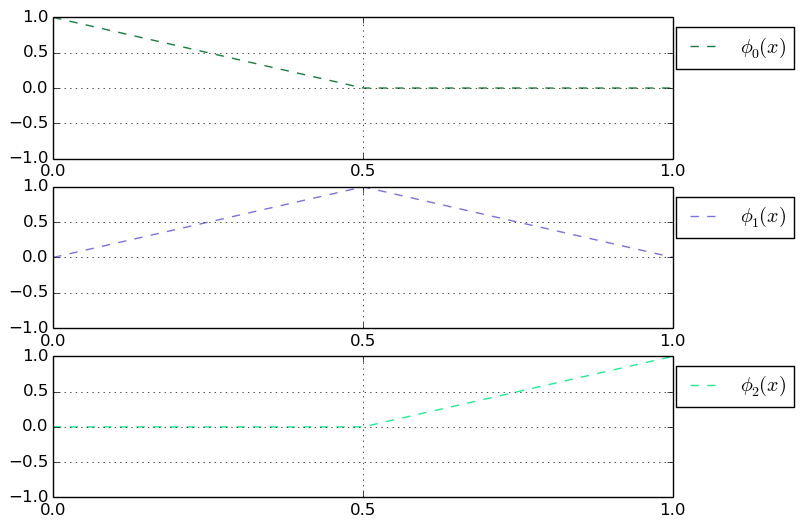
\includegraphics[width=1\textwidth, center]{figuras/phis_elementos_finitos.png}
    
  \end{minipage}
\end{SCfigure}
%\pagebreak \\
 Um exemplo desse domínio dividido em dois é:
\begin{figure}[h]
 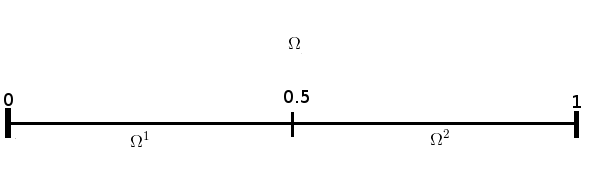
\includegraphics[width=0.45\textwidth, center]{figuras/2_elementos_finitos.png}
\caption{Domínio $\Omega$ dividido em dois elementos $\Omega_e$}
 \end{figure}\\
 A maneira de satisfazer a condição de fronteira de \emph{Dirichlet} para \emph{x=0} é fazer $u(x_0) = g_D$, assim, decompomos $u^\delta$ em $u^\delta = u^H + u^D$, fazendo:
 \begin{align}
 & u^H = \hat{u_1}\phi_1(x) + \hat{u_2}\phi_2(x)
 & u^D = g_D\phi_0(x)
 \end{align}
 onde $\hat{u_0}\ e \hat{u_1}$ são arbitrários. A aproximação definida em $u^H$ contém as mesmas funções usadas na função teste $v$, tendo :
 \begin{equation}
 v^\delta(x) = \hat{v_1}\phi_1(x) + \hat{v_2}\phi_2(x)
 \end{equation}
 tanto $\hat{v_0}$ e $\hat{v_1}$ são \emph{desconhecidos}. Definimos $f(x)$ como uma expansão idêntica de $u^\delta$ em relação a $\phi$:
 \begin{equation}
 f(x) = \sum^2_{i=0} \hat{f_0}\phi_0(x) +\hat{f_1}\phi_1(x) + \hat{f_2}\phi_2(x)
 \end{equation}
 Caso $f$ seja constante ou linear, então a aproximação é exata. Para funções algo mais complexo, os coeficientes $\hat{f_0},\hat{f_1},\hat{f_2}$, tem que ser determinada e podem ser escolhidas como  $\hat{f_0} = f(0),\hat{f_1} = f(0.5),\hat{f_2} = f(1)$.

 Definidos $u$,$v$,$f$ podemos calcular cada termo na equação \eqref{eq:weakform}:
 primeiro termo:
\begin{align}
\int^1_0 \frac{\partial v^\delta}{\partial x} \frac{\partial u^\delta}{\partial x} \partial x\ & = \int^{\frac{1}{2}}_0 (2\hat{v_1})(2\hat{u_1}) \partial x + \int^1_{\frac{1}{2}} (-2\hat{v_1}+2\hat{v_2})(-2\hat{u_1}+2\hat{u_2}) \partial x \\
& = [\hat{v_1}\ \ \hat{v_2} ]\begin{bmatrix}
4 & -2 \\ 
-2 & 2
\end{bmatrix}
\begin{bmatrix}
\hat{u_1}\ \\ \hat{u_2}\\ 
\end{bmatrix}
\end{align}
 segundo termo:
\begin{align}
\int^1_0v^\delta f\ \partial x = & \int^{\frac{1}{2}}_0 (2\hat{v_1}x)(\hat{f_0}(1-2x) + \hat{f_1}(2x) \partial x + \\
& \int^1_{\frac{1}{2}} (\hat{v_1}2(1-x) +\hat{v_2}(2x-1))(\hat{f_1}2(1-x) +\hat{f_2}(2x-1)) \partial x \\
& [\hat{v_1}\ \hat{v_2}]\begin{bmatrix}
\frac{1}{12}\hat{f_0} + \frac{1}{3}\hat{f_1} + \frac{1}{12}\hat{f_2} \\ 
\frac{1}{12}\hat{f_0} + \frac{1}{6}\hat{f_2}
\end{bmatrix}
\end{align}
 terceiro termo:
\begin{equation}
v^\delta(1)g_n = (\hat{v_1}\phi_1(1) + \hat{v_2}\phi_2(1))g_N = [\hat{v_1} \ \hat{v_2}]\begin{bmatrix}
0\\ 
1
\end{bmatrix}g_n
\end{equation}
 quarto termo:
 \begin{align}
  \int^1_0 \frac{\partial v^\delta}{\partial x}\frac{\partial u^\delta}{\partial x} &= \int^{\frac{1}{2}}_0 (2\hat{v_1})(-2g_D)\ \partial x \\
             &=  [\hat{v_1}\ \hat{v_2}]\begin{bmatrix}
-2g_D\\ 
0
\end{bmatrix}
 \end{align}
 Assim temos que na equação \eqref{eq:weakform}, substituindo cada termo e botando $[\hat{v_1}\ \hat{v_2}]$ em evidência, temos:
\begin{align}
[\hat{v_1}\ \hat{v_2}]\begin{Bmatrix}
\begin{bmatrix}
4 & -2 \\ 
-2 & 2
\end{bmatrix}
\begin{bmatrix}
\hat{u_1}\ \\ \hat{u_2}\\ 
\end{bmatrix}
-
\begin{bmatrix}
\frac{1}{12}\hat{f_0} + \frac{1}{3}\hat{f_1} + \frac{1}{12}\hat{f_2} \\ 
\frac{1}{12}\hat{f_0} + \frac{1}{6}\hat{f_2}
\end{bmatrix}-
\begin{bmatrix}
0\\ 
g_n
\end{bmatrix}+
\begin{bmatrix}
-2g_D\\ 
0
\end{bmatrix}
\end{Bmatrix}
\end{align}
 Assim, notamos que para quaisquer $[\hat{v_1},\ \hat{v_2}]$,podemos solucionar essa equação, apenas resolvendo a equação dentro dos \emph{colchetes},fazendo $g_D$ e $g_N$ ambos iguais a $1$, temos:
\begin{equation}
 \begin{bmatrix}
\hat{u_1}\ \\ \hat{u_2}\\ 
\end{bmatrix}
= \begin{bmatrix}\frac{3}{2} +\frac{1}{24}\hat{f_0}+\frac{5}{24}\hat{f_1}+\frac{1}{8}\hat{f_2} \\ 2 +\frac{1}{24}\hat{f_0}+\frac{1}{4}\hat{f_1}+\frac{5}{24}\hat{f_2} \end{bmatrix}
\end{equation}
 Calculados $\hat{u_1},\ \hat{u_2}$, podemos fazer a aproximação por elementos finitos, $u^\delta =g_D\phi_0(x) + \hat{u_1}\phi_1(x) +\hat{u_2}\phi_2(x)$, temos:
\begin{equation}
u^\delta =
\begin{cases}
1 + x +\frac{x}{12}\hat{f_0} + \frac{5x}{12}\hat{f_1} +\frac{x} {4}\hat{f_2},\ \ 0 \leq x \leq \frac{1}{2}\\
1 + x +\frac{1}{24}\hat{f_0} + \frac{2+x}{12}\hat{f_1} +\frac{1+4x}{24}\hat{f_2},\ \ \frac{1}{2} \leq x \leq 1
\end{cases}
\end{equation}



\subsection{Forma Matricial do problema}
	Ao decidir resolver a equação diferencial, obtemos um sistema de equações diferenciais para cada função teste $v_j^\delta$  e sem perder a igualdade transformamos o problema diferencial em um problema variacional, segue o exemplo abaixo :
\begin{align}
\frac{\partial^2 u^\delta }{\partial x^2} + \lambda u^\delta &= f\\[1.5pt]
v^\delta_j (\frac{\partial^2 u^\delta }{\partial x^2} + \lambda v^\delta_j\ u^\delta) \ &= v^\delta_j f\\[1.5pt]
\int_\Omega v^\delta_j (\frac{\partial^2 u^\delta }{\partial x^2} + \lambda v^\delta_j\  u^\delta) \partial x &= \int_\Omega v^\delta_j  f \partial x\\[1.5pt]
\int_\Omega v^\delta_j \frac{\partial^2 u^\delta }{\partial x^2}\ \partial x + \int_\Omega \lambda v^\delta_j\ u^\delta\partial x &=\ \int_\Omega v^\delta_j  f \partial x\\[1.5pt]
\int_\Omega \frac{\partial v^\delta_j }{\partial x} \frac{\partial u^\delta }{\partial x}\ \partial x + \int_\Omega \lambda v^\delta_j\ u^\delta\ \partial x - (v^\delta_j  \frac{\partial u^\delta }{\partial x})\Biggm\lvert_\Omega\ &=\  \int_\Omega v^\delta_j\  f\ \partial x \ \forall j = 1,2,3,\dots,N 
\end{align}
 Como $u^\delta$ é a aproximada de $u$ utilizando a função teste $v^\delta_j$, temos:
\begin{align}
\sum^N_{i=1} u_i \int_\Omega \frac{\partial v^\delta_j }{\partial x} \frac{\partial v^\delta_i }{\partial x}\ \partial x +\sum^N_{i=1} u_i  \int_\Omega \lambda\ v^\delta_j v^\delta_i \ \partial x =\  (v^\delta_j  \frac{\partial u^\delta }{\partial x})\Biggm\lvert_\Omega + \int_\Omega v^\delta_j\ f\ \partial x \ \forall j =1,2,\dots,N 
\end{align}  
Como essa equação é definida para todo  $v_j$ para $j = 1,2,\dots,N$, podemos reescrever de forma matricial, onde $(v^\delta_j  \frac{\partial u^\delta }{\partial x})\Biggm\lvert_\Omega$ só é adicionado ao lado direito quando  há uma condição de \emph{Neumann} e quando  $v^\delta_j$ é diferente de zero nos extremos do domínio. Assim, podemos reescrever o sistema como:
\begin{equation}
\{ M + \lambda S\} U = F
\end{equation}
 Onde chamamos a matriz M de matriz de massa e S de matriz de rigidez.
\begin{align}
M &=
\begin{bmatrix}
\int_\Omega \frac{\partial v^\delta_{1}}{\partial x}\frac{\partial v^\delta_{1}}{\partial x}\ \partial x  & \int_\Omega \frac{\partial v^\delta_{1}}{\partial x}\frac{\partial v^\delta_{2}}{\partial x}\ \partial x  & \dots & \int_\Omega \frac{\partial v^\delta_{1}}{\partial x}\frac{\partial v^\delta_{N}}{\partial x}\ \partial x  \\ 
\int_\Omega \frac{\partial v^\delta_{1}}{\partial x}\frac{\partial v^\delta_{2}}{\partial x}\ \partial x  & \int_\Omega \frac{\partial v^\delta_{2}}{\partial x}\frac{\partial v^\delta_{2}}{\partial x}\ \partial x  & \dots & \int_\Omega \frac{\partial v^\delta_{2}}{\partial x}\frac{\partial v^\delta_{N}}{\partial x}\ \partial x  \\ 
\vdots & \vdots & \vdots & \dots \\
\int_\Omega \frac{\partial v^\delta_{N}}{\partial x}\frac{\partial v^\delta_{1}}{\partial x}\ \partial x  & \int_\Omega \frac{\partial v^\delta_{N}}{\partial x}\frac{\partial v^\delta_{2}}{\partial x}\ \partial x  & \dots & \int_\Omega \frac{\partial v^\delta_{N}}{\partial x}\frac{\partial v^\delta_{N}}{\partial x}\ \partial x  \\ 
\end{bmatrix}, \\
S &= \begin{bmatrix}
\int_\Omega v^\delta_1 v^\delta_1 \partial x & \int_\Omega v^\delta_1 v^\delta_2 \partial x & \dots & \int_\Omega v^\delta_1 v^\delta_N \partial x \\ 
\int_\Omega v^\delta_2 v^\delta_1 \partial x & \int_\Omega v^\delta_2 v^\delta_2 \partial x & \dots & \int_\Omega v^\delta_2 v^\delta_N \partial x\\ 
\vdots & \vdots & \ddots & \vdots \\
\int_\Omega v^\delta_N v^\delta_1 \partial x & \int_\Omega v^\delta_N v^\delta_2 \partial x & \dots & \int_\Omega v^\delta_N v^\delta_3 \partial x
\end{bmatrix},\
U = \begin{bmatrix}
u_1\\ 
u_2\\ 
\vdots \\
u_N
\end{bmatrix}\\
F &= \begin{bmatrix}
\int_\Omega v^\delta_1\ f\ \partial x +  (v^\delta_1  \frac{\partial u^\delta }{\partial x})\Biggm\lvert_\Omega \\ 
\int_\Omega v^\delta_2\ f\ \partial x +  (v^\delta_2  \frac{\partial u^\delta }{\partial x})\Biggm\lvert_\Omega \\ 
\vdots \\
\int_\Omega v^\delta_N\ f\ \partial x +  (v^\delta_N  \frac{\partial u^\delta }{\partial x})\Biggm\lvert_\Omega\\ 
\end{bmatrix}
\end{align}

%\pagebreak

 
\subsection{Mapeamento}
 Quando tratamos das funções de bases, temos as funções globais e as locais. Apesar das funções globais serem na teoria usadas para o calcular as matrizes de \emph{massa} e de \emph{rigidez}, na prática decompomos as funções globais em elementos e utilizamos dessa decomposição as funções de base locais para o cálculo das matrizes.\\
 Tomemos como exemplo as funções lineares globais $\Phi$ em um domínio $\Omega = \{x\ |\ 0\leq x \leq 1\}$ subdividido em \emph{3} elementos. Temos 4 graus de liberdade nessa expansão, definida no máximo em 2 elementos ao mesmo tempo,que vale 1 em um dos extremos desses elementos e decresce para 0 para o em direção aos outros extremos.
\begin{equation}
\Phi_1(x) = \left\{\begin{matrix}
1 - 3x,\ 0 \leq x \leq \frac{1}{3}\\
0\ , \frac{1}{3} < x \leq 1
\end{matrix}\right.\ \ 
\Phi_2(x) = \left\{\begin{matrix}
3x,\ 0 \leq x \leq \frac{1}{3}\\
2 - 3x\ , \frac{1}{3} < x \leq \frac{2}{3}\\
0\ , \frac{2}{3} < x \leq 1
\end{matrix}\right.\\
\end{equation} 
\begin{equation}
\Phi_3(x) = \left\{\begin{matrix}
0 ,\ 0 \leq x < \frac{1}{3}\\
3x - 1\ ,\ \frac{1}{3} < x \leq \frac{2}{3}\\
-3x + 3 \ ,\ \frac{2}{3} < x \leq 1
\end{matrix}\right.\\
\Phi_4(x) = \left\{\begin{matrix}
0\ ,\ \ 0 \leq x < \frac{1}{3}\\
0\ ,\ \frac{1}{3} < x \leq \frac{2}{3}\\
3x -2 \ ,\ \frac{2}{3} < x \leq 1
\end{matrix}\right.
\end{equation}

\begin{figure}[!h]
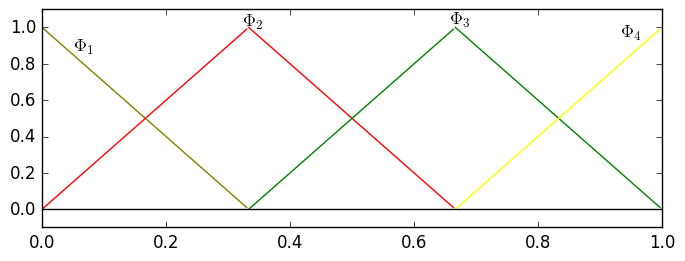
\includegraphics[width=0.6\textwidth, center ]{figuras/Matrix_elem_global.png}
\caption{funções globais para cada elemento}
\end{figure}

Também podemos definir funções locais $\phi^e_p(x)$ onde $\Omega_e = \{x \| x_{e1} \leq x \leq x_{e2} \}$:
\begin{equation}
\phi^e_1\ = \left\{\begin{matrix}
\frac{x_{e1}\ -\ x}{x_{e2} - x_{e1}}, x \in \Omega_e \\
0 ,\ x \notin \Omega_e 
\end{matrix}\right.
\phi^e_2\ = \left\{\begin{matrix}
\frac{x\ -\ x_{e1}}{x_{e2} - x_{e1}}, x \in \Omega_e \\
0 ,\ x \notin \Omega_e 
\end{matrix}\right.
\end{equation} 

\begin{figure}[!h]
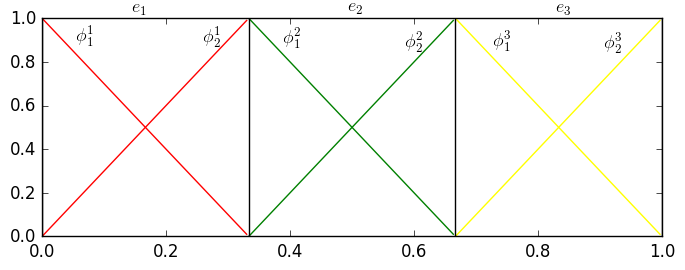
\includegraphics[width=0.6\textwidth, center ]{figuras/Matrix_element_local.png}
\caption{funções locais para cada elemento}
\end{figure}
 Podemos remapear $\Phi_i$'s em função das $\phi_i$'s locais como:
\begin{align}
\Phi_1 &= \phi_{1}^{1} \\[0.5pt]
\Phi_2 &= \phi_{2}^{1} + \phi_{1}^{2} \\[0.5pt]
\Phi_3 &= \phi_{2}^{2} + \phi_{1}^{3} \\[0.5pt]
\Phi_4 &= \phi_{2}^{3}
\end{align}

\begin{equation}
\begin{bmatrix}
\phi_1^1\\[1.9pt] 
\phi_2^1\\[1.9pt]
\phi_1^2\\[1.9pt] 
\phi_2^2\\[1.9pt]
\phi_1^3\\[1.9pt] 
\phi_2^3\\[1.9pt] 
\end{bmatrix}\ = \
\begin{bmatrix}
1 &0  & 0 & 0 \\ 
0 & 1 & 0 & 0\\ 
0 & 1 & 0 & 0\\ 
0 &0  & 1 & 0\\ 
0 &0  & 1 & 0\\ 
0 &0  & 0 & 1
\end{bmatrix}\
\begin{bmatrix}
\Phi_1\\ 
\Phi_2\\ 
\Phi_3\\ 
\Phi_4
\end{bmatrix}
\end{equation}

Notamos que existe uma relação entre as funções  $\Phi$ globais e as $\phi$ locais, para tal existe uma matriz $A$ que nos permite igualá-las, porém a relação inversa que nos mais interessa, na qual podemos fazer operações locais em cada elemento. Essa relação nos é interessante pois na formulação de Galerkin, nos permite fazer os cálculos das integrais localmente.
\begin{equation}
\int_\Omega\ \Phi_2(x) \partial x = \int_{0}^{\frac{1}{3}} \phi^1_2(x) \partial x + \int_{\frac{1}{3}}^{\frac{2}{3}} \phi^2_1(x)\ u(x) \partial x
\end{equation}

Devido ao fato da matriz $A$ ser uma matriz esparsa e portanto numericamente ineficiente para ser usada como um operador, utilizamos outra saída. Essa alternativa é uma matriz \emph{map}eadora em que cada coluna é um elemento (e) e cada linha o indice da função global (i).
\begin{equation}
map[1,i]= \begin{bmatrix}
1\\
2
\end{bmatrix},\
map[2,i]= \begin{bmatrix}
2\\
3
\end{bmatrix}\
,map[3,i]= \begin{bmatrix}
3\\
4
\end{bmatrix}
\end{equation}

usando um pseudo código, utilizamos essa matriz mapeadora para montar a função global dada a local:
\begin{lstlisting}
 for e =1:Nel
 	for i=1,2
 		$\Phi$[map[e,i]] = $\Phi$[map[e,i]] + $\phi$[e,i]
 	end
 end
\end{lstlisting}
Assim a matriz de massa \emph{global} $M$ definida como $M_{ij} = \int_\Omega \Phi_i\ \Phi_j \partial x$ analogamente como  o código anterior, pode ser reescrita a função de uma matriz de massa $M^e$ \emph{local}, utilizando uma matriz de mapeamento $map$ similar a anterior.
\begin{figure}[!h]
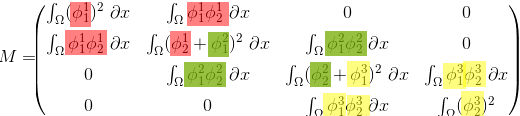
\includegraphics[width=0.6\textwidth, center ]{figuras/Matrix_element.png}
\caption{Matriz de massa mapeada}
\end{figure}
 Com o exemplo anterior conseguimos ter uma idéia de como remapear as respectivas matrizes para funções lineares, porém utilizando polinômios de maior grau podemos usar o mesmo código para essa reestruturação. Sendo assim podemos usar polinômios de Lagrange, Legendre ou mesmo uma nova base da família do polinômio de Jacobi para obter assim solucionar problemas mais complexos que não poderíamos solucionar com uma função linear.

\section{Condensação estática}
  Após o mapeamento das matrizes temos então a tarefa de resolver o sistema linear.Utilizando o fato do mapeamento ter separado as funções de base para os modos \textbf{internos} (i) e os modos de \textbf{fronteira} (b) de cada elemento, aplicamos a técnica de \emph{condensação estática}. Onde com remapeando os vetores x e f do sistema linear $A\  x = f$ de maneira a ficar primeiro os coeficientes de fronteira e depois os coeficientes internos temos o sistema reescrito como:
  \begin{equation}
    x = \left\{\begin{matrix} x_b \\ x_i \\ \end{matrix}\right\}\ ,\ f =  \left\{\begin{matrix} f_b \\ f_i \\ \end{matrix}\right\}\
  \end{equation}
E com o remapeamento feito anteriormente, temos a matriz A global como:
\begin{figure}[H]
\centering
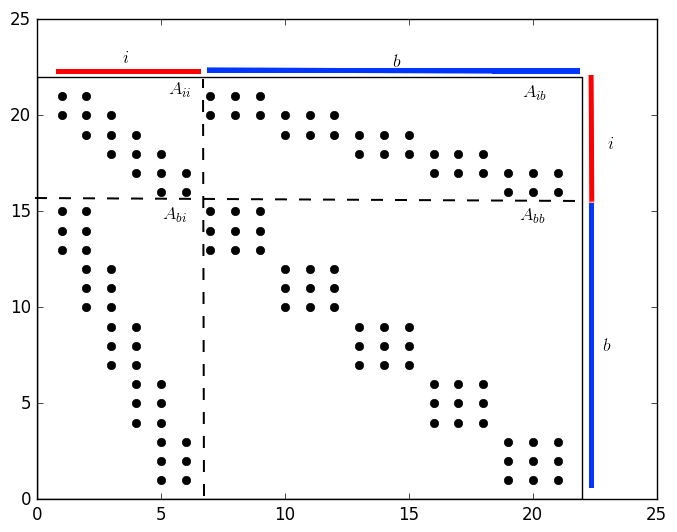
\includegraphics[width=0.7\textwidth,center]{figuras/Matriz_global.png}
\caption{esquema da matriz global remapeada} 
\end{figure}
onde cada $A_{\cdot \cdot}$ é uma sub matriz de A em que $A_{ii}$ é uma matriz em banda, $A_{ib}$ e $A_{bi}$ são  matrizes esparsas e $A_{bb}$ é uma matriz em bloco.

\begin{equation}
A\cdot x  = \left[ 
\begin{matrix} 
A_{bb} & A_{bi} \\
A_{ib} & A_{ii} \\
\end{matrix}\right] \cdot \left\{
\begin{matrix} x_b \\ x_i \\ 
\end{matrix}\right\} = 
\left\{\begin{matrix} f_b \\ f_i \\\end{matrix}\right\} 
\end{equation}
Para resolver esse sistemas fazemos:
\begin{equation}
x_i = A_{ii}^{-1} f_i - A_{ii}^{-1} A_{ib} x_b
\end{equation}
Que substituindo $x_i$ na equação de  $x_b$, obtemos:
\begin{equation}
\left( A_{bb} - A_{bi}A_{ii}^{-1} A_{ib} \right) x_b = f_b - A_{bi}A_{ii}^{-1} f_i\\
A'_{bb} \cdot x_b = f'_b
\end{equation}
onde:
\begin{align}
& A'_{bb} = A_{bb} - A_{bi}A_{ii}^{-1} A_{ib}\\ 
& f'_b = f_b - A_{bi}A_{ii}^{-1} f_i
\end{align}
Assim, utilizando o remapeamento e a condensação estática, encontramos $x_b$ e $x_i$ da equação.

